\section{Diffusione}\label{diffusione}

Per diffusione si intende il \textit{trasporto di materia dovuto al moto molecolare del mezzo in cui essa è immersa} \cite{salsa}. Gli atomi e le molecole di cui sono composti i fluidi sono in continuo movimento casuale: questo fenomeno è chiamato \textit{agitazione termica} perché dipende dalla temperatura. Dalla termodinamica statistica si sa che l'energia cinetica di una particella di massa $m$ e velocità $v$ dipende dalla temperatura $T$ proporzionalmente alla costante di Boltzmann\footnote{$k_B = 1.38\cdot10^{-23} J/K$} $k_B$ secondo la relazione:
$$E_{cin}= \frac{1}{2}mv^2 = \frac{3}{2}k_B T$$
Come si può osservare la velocità delle molecole aumenta all'aumentare della temperatura e, in un mezzo a temperatura costante, è inversamente proporzionale al loro peso molecolare. Bisogna fare attenzione a non confondere questa velocità, che è di tipo vibrazionale, con la velocità media di percorrenza dello spazio, o velocità di diffusione; quest'ultima infatti, a causa dei continui urti e deviazioni che la molecola subisce, è molto più piccola della velocità vibrazionale dovuta all'agitazione termica. A titolo esemplificativo, in acqua a $20^{\circ} C$  la molecola di ossigeno ha una velocità di diffusione di circa $1$ $mm/s$ a fronte di una velocità vibrazionale di circa $5$ $m/s$ \cite{fisica}.

Il fenomeno della \textit{diffusione libera} si ha quando il soluto diffonde liberamente a seguito dell'agitazione termica; questo fenomeno è descritto dalla legge di Fick:
\begin{equation}\label{fick1}
	\phi_d = - D \frac{\Delta C}{\Delta x}
\end{equation}
in cui $\phi_d $ è il flusso diffusivo di soluto attraverso la membrana, reale o virtuale, di spessore $\Delta x$; $D$ è la diffusività del mezzo in cui avviene la diffusione. Il coefficiente $D$ dipende principalmente dalla temperatura assoluta, ma anche dal tipo di urti che si instaurano tra molecole di soluto e molecole di solvente, e quindi dalle caratteristiche chimico-fisiche delle specie interagenti. La più semplice relazione per $D$ è la formula di \textit{Einstein-Stokes} valida per particelle che si muovono in un mezzo viscoso:
$$D = \frac{k_B T}{6 \pi \eta r}$$
dove $r$ è il raggio efficace del soluto e $\eta$ la viscosità del solvente. Il coefficiente di diffusione attraverso una membrana può essere messo in relazione con quello libero considerando che la molecola di raggio efficace $r$, per attraversare la membrana, deve introdursi in uno dei suoi pori di raggio $R$ senza urtarne il bordo (altrimenti rimbalzerebbe tornando indietro). Questo fa sì che, come mostra la \figurename~\ref{hindrance}a, l'area efficace di ingresso nel poro non sia $\pi R^2$ ma:
$$\pi(R-r)^2 = \pi R^2\biggl(1-\frac{r}{R}\biggr)^2 = \pi R^2 \varepsilon_1$$
dove il coefficiente $\varepsilon_1$ è il fattore correttivo che tiene conto della geometria del poro e della molecola. Un ulteriore limitazione alla diffusione è data dall'urto delle molecole con le pareti interne del poro (\figurename~\ref{hindrance}b) che riduce ancora il coefficiente $D$ di un fattore $\varepsilon_2$ anche esso funzione della geometria degli urti\footnote{da relazioni sperimentali \cite{costantino} si ricava che $\varepsilon_2 = 1-2.1\cdot R/r + 2.09 \cdot (R/r)^3 - 0.95 \cdot (R/r)^5$.}. Ambedue i fattori $\varepsilon_1$ e $\varepsilon_2$ possono essere inglobati in un unico fattore $\varepsilon$ detto di \textit{hindrance}\footnote{in termini statistici, il fattore di \textit{hindrance} rappresenta la probabilità che una molecola attraversi il poro della membrana.} per giungere alla relazione:
$$D_p = \varepsilon_1 \varepsilon_2 D = \varepsilon D$$ 
\begin{figure}[htb]
	\centering
	\subfigure[]%
	{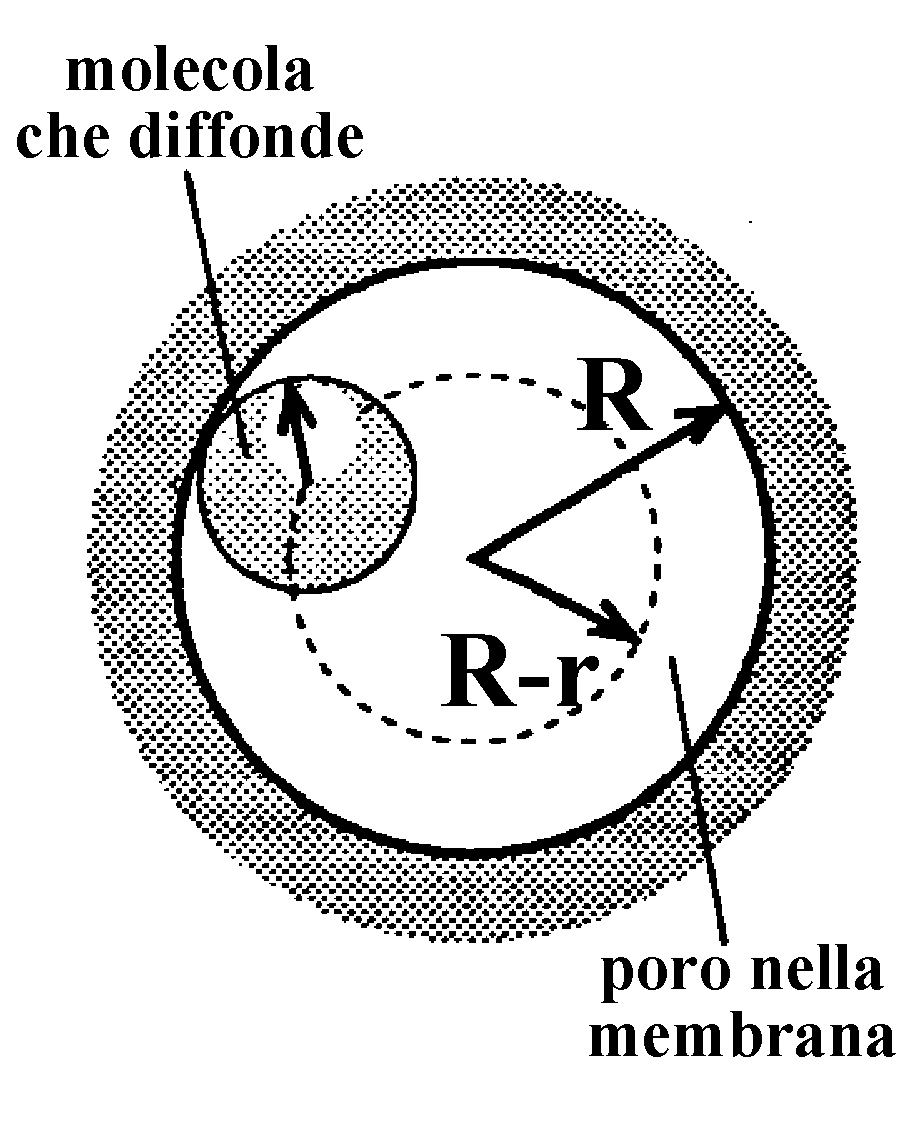
\includegraphics[width=0.25\textwidth]{immagini/hindrance1.eps}}\qquad
	\subfigure[]%
	{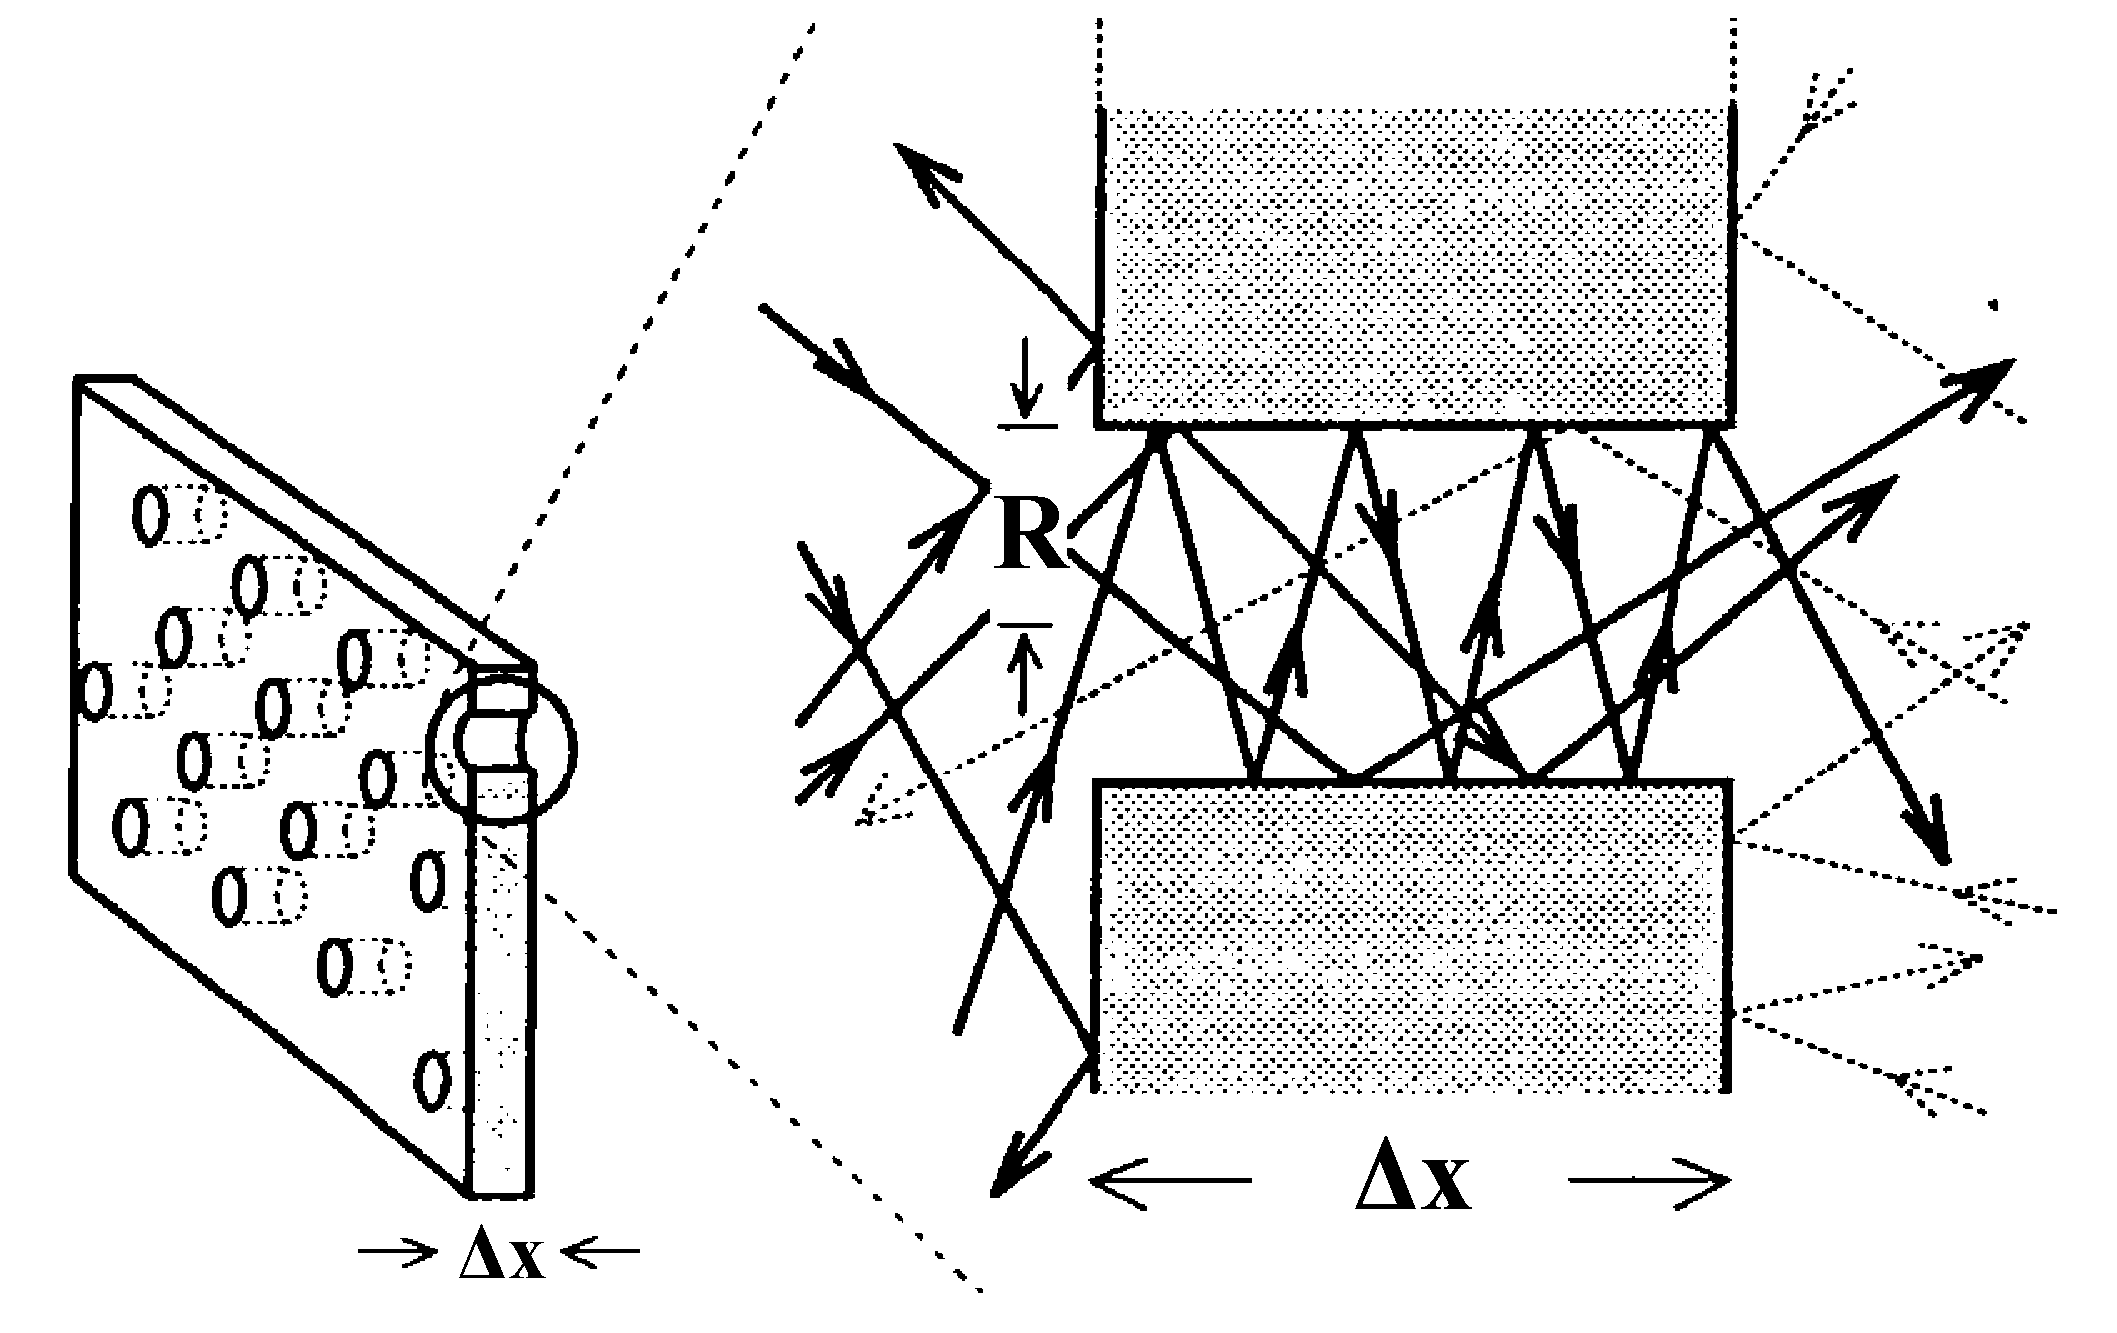
\includegraphics[width=0.6\textwidth]{immagini/hindrance2.eps}}
		\caption{(a) Il centro di una molecola sferica di raggio $r$, perché questa possa penetrare nel poro di raggio $R$, deve trovarsi all'interno della circonferenza tratteggiata di raggio $(R-r)$. (b) Una volta che la molecola è penetrata nel poro urta le pareti interne per cui le proprietà diffusive all'interno della membrana risultano differenti da quelle all'esterno.}\label{hindrance}
\end{figure}
Il coefficiente $D_p$ così ricavato è il coefficiente di diffusione libera attraverso il singolo poro della membrana, che, a causa della geometria di pori e molecole coinvolte nella diffusione, è minore di quello di diffusione libera nel solvente. Se ora si vuole ricavare il coefficiente $D_m$ di diffusione dell'intera membrana a partire da quella del singolo poro, è necessario considerare la frazione di volume effettivo $\alpha$ che le molecole hanno a disposizione per diffondere. Effettuando le sostituzioni opportune, l'equazione \ref{fick1} diventa:

\begin{equation}\label{phiD}
	\phi_d = - \varepsilon D \frac{\alpha\Delta C}{\Delta x} = - D_p \frac{\alpha\Delta C}{\Delta x} =  -D_m \frac{\Delta C}{\Delta x} = -P_m \Delta C
\end{equation}
\noindent
\newline
in cui $D_m = \alpha D_p$, e $P_m = D_m/\Delta x$ è chiamato coefficiente di \textit{permeabilità} della membrana. Le unità di misura di $\phi_d$ sono $[mol \cdot s^{-1}]$ e il pedice $d$ indica che il trasporto è di tipo diffusivo.